\section*{Синтез и построение полусуматора}
\addcontentsline{toc}{section}{Синтез и построение сумполусуматораматора}
\subsection*{Построение полусумматора}
\addcontentsline{toc}{subsection}{Построение полусумматора}

Для синтеза модели полусумматора необходимо составить аналитическую модель 
посредством построения СДНФ для управляющих сигналов S и P из таблицы \ref{table:1}. \par

\begin{table}[h!]
    \begin{center}
        \begin{tabular}{ | m{1cm} | m{1cm} | m{1cm} | m{1cm} | }
            \hline
            X & Y & S & P \\ \hline
            0 & 0 & 0 & 0 \\ \hline 
            0 & 1 & 1 & 0 \\ \hline
            1 & 0 & 1 & 0 \\ \hline
            1 & 1 & 1 & 1 \\ \hline
        \end{tabular}
        \caption{Таблицы истинности полусумматора}
        \label{table:1}
    \end{center}    
\end{table}

В результате получаем две функции описывающие управляющие сигналы S и P, 
где S - это результат суммирования; P - перенос в старший разряд.
\begin{itemize}
    \item $S=\overline{X}Y \cup X\overline{Y}$
    \item $P=XY$
\end{itemize}

На основании полученных выражений составим модель полусуматора в Multisim 
(рис. \ref{image:1}).

\begin{figure}[h]
    \centering
    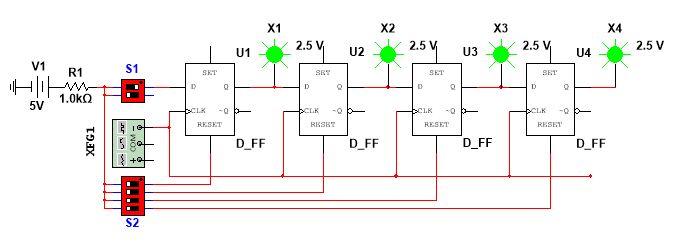
\includegraphics[scale=0.8]{image-1.png}
    \caption{Модель полусумматора}
    \label{image:1}
\end{figure}

\newpage
\subsection*{Тестирование полусуматора}
\addcontentsline{toc}{subsection}{Тестирование полусуматора}
Управляющие сигналы полусуматора подключены к ламповым индикаторам. 
При подаче входных сигналов в соответсвие с таблицей \ref{table:1} ожидаем корректную индикацию 
ламп управляющих сигналов. Проверим работу полусуматора для набора $X=1,Y=0$. 
Ожидаем индикацию сигнала S. \par

\begin{figure}[h]
    \centering
    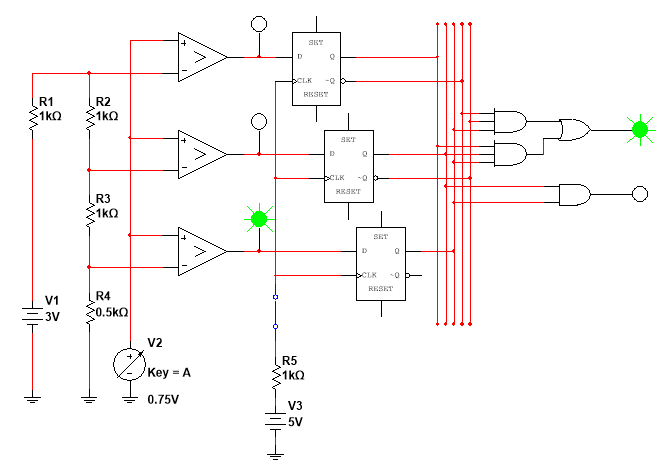
\includegraphics[scale=0.8]{image-2.png}
    \caption{Проверка работы полусумматора}
    \label{image:2}
\end{figure}

Результат соответвует ожиданию. Аналогично были проверены остальные наборы входных сигналов.